\section{Proposed Research}
% Including method or approach and expected difficulties
% This must constitute about 50\% of the text of the written proposal: 7-8 pages
% Clear statement of the work to be undertaken and must include:
% Objectives for the period of the proposed work and expected significance
% Relation to the present state of knowledge in the field and to work in progress at Michigan/elsewhere
% Expected research program sequence
% Decision points expected during the course of the research
% Methods of data reduction, evaluation, interpretation and presentation

% https://en.wikipedia.org/wiki/Folding_funnel#/media/File:Folding_funnel_schematic.svg
\begin{figure}[t]
\begin{center}
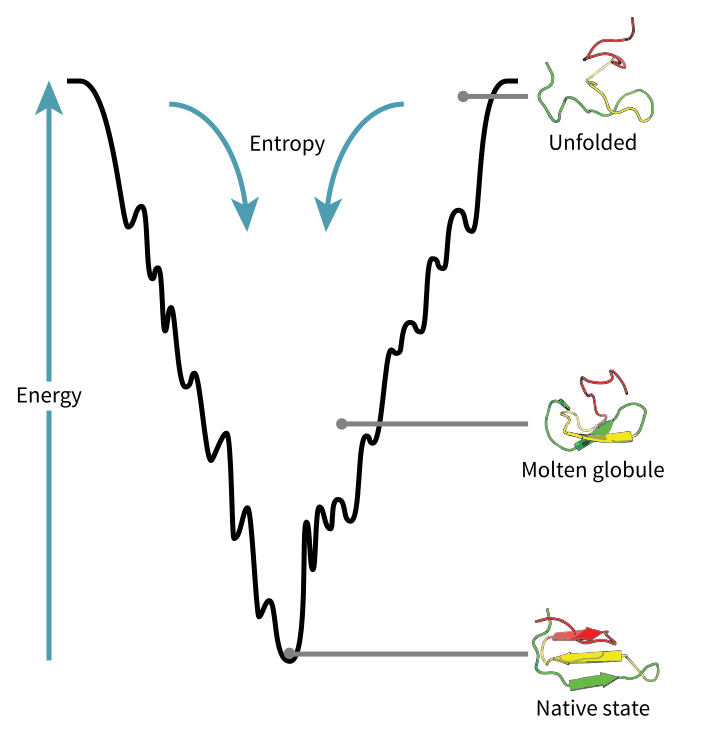
\includegraphics[width=3in]{../figures/foldingfunnel.png}
\caption{The diagram sketches how proteins fold into their native structures by minimizing their free energy. (Source: Wikipedia}
\label{fig:funnel}
\end{center}
\end{figure}

\subsection{Model background}
For our system, we use nets of the 5 Platonic shapes as described in \cite{Dodd_2018_unpublished}.
These nets are implemented as rigid bodies with harmonic springs.
Edges of each net ``face'' have non-specific attractive patches.
Molecular dynamics (implemented in HOOMD-blue \cite{HOOMD_2008, HOOMD_2015}) is used to simulate assembly in the canonical (NVT) ensemble.

In a forth-coming study from the Glotzer lab using this system \cite{Dodd_2018_unpublished}, the authors find that for the same target shape, compact nets with few leaves assemble most reliably (in agreement with \cite{Azam_2009_PlosOne}.
By investigating the assembly behavior for shapes with fewer possible net constructions (ADD), they are then able to use these features to predict which nets will assemble for shapes with a wide variety of possible net constructions. 
Additionally, they observe that reliable assembly is due to the formation of local native (that is, present in the final structure) bonds early in the simulation which in turn bring non-local contacts together to be folded next (i.e. cooperatively) \cite{Dill_1993_PNAS}.
They posit that as each net folds, it freezes out the fewest possible number of degrees of freedom, thereby maximizing the conformational entropy along the folding pathways.

This finding closely mirrors what is already know in studies of protein folding.
In 1968, Cyrus Levinthal posed the following thought experiment, come to be known as ``Levinthal's Paradox'' \cite{Levinthal_1969}.
Even at that time, proteins were known to assemble in less than a second.
However, if proteins explored all their possible degrees of freedom they would never be able to assemble.
A polypeptide with 100 residues would have 99 peptide bonds, and therefore 198 different phi and psi bond angles.
If each of those bond angles could be in one of three stable conformations, the protein would potentially have to sample $3^{198}$ different conformations to reach its native configuration.
Randomly sampling such a large number of configurations in search of the native configuration is not even possible in the life-time of the universe-- and thus, Levinthal's Paradox.

Levinthal posited that biological folding times could be explained by the formation of local, native contacts which would stabilize the structure and ``serve as nucleation points in the folding process''.
Indeed, over 20 years later, these small biases (on the order of just a few $kT$) towards the native configuration were mathematically demonstrated to result in biologically realistic protein folding times \cite{Zwanzig_1992_PNAS,Martinez_2014_JChemEd}.
In analyses of real-world folding times, protein folding speeds correlate with the topology of the native protein.
Fast folders usually have mostly local structure, such as helices and tight turns, whereas slow folders usually have more non-local structure, such as $\beta$-pleated sheets \cite{Plaxco_1998_JMolBio}.

Further work on elucidating experimental protein kinetics detected the partially folded intermediates transition states in the folding process posited by Levinthal \cite{Dill_2007_CurrOpinStructBio}. 
Statistical mechanical models of protein folding uncovered that assembly does not follow single microscopic pathway.
Instead, protein folding is characterized by funnel-shaped energy landscapes, with entropy increasing as proteins assemble with decreasing free energy as shown in Figure \ref{fig:funnel} \cite{Dill_1997_Nature}.

However, low free energies of a target structure do not guarantee efficient assembly.
One particularly clarifying way of seeing this is through disconnectivity graphs developed by David Wales and colleagues \cite{Wales_2017_JChemPhys}.
\textcolor{red}{(Describe disconnectivity graphs here and how they're used.)}

\textcolor{red}{(Jacobs-- worth talking about protein contact maps here?)}

Given that we are able to replicate complex findings from protein folding in this simple system, this suggests that we can continue to use this system as a toy model for developing theory of tailored self-assembly.
Levinthal posited that some local contacts may act as ``nucleation points in the folding process''.
Can we identify similar critical bonds in foldings of nets?
Is it possible to change the folding propensity of a ``bad folding'' net by seeding the net with a critical bond?

This second question follows from theories in origami. 
Why is it important that we find these most-critical self-assembly ``seeds''?
Origami theory is developed for a system a zero temperature-- that is, developing theories to avoid needing to back-track along an assembly pathway (e.g. after encountering a local-minima) are desirable.
In a class of NP-hard satisfiability (SAT) problems, careful seeding of the search for global minima has been shown to greatly reduce or even eliminate backtracking \cite{Stern_2017_arxiv}(10) before reaching the global minima \cite{Stern_2017_arxiv}(43).
(Fun fact: this includes filling in the right boxes first in a game of Sudoku \cite{Stern_2017_arxiv}(43).) 

\textcolor{red}{Check \cite{Stern_2017_arxiv}(43) for good intro on origami and self-assembly}.

%=====
%ADDITIONAL THOUGHTS TO INCLUDE
%=====
\subsection{Proposed projects}

Nature is very good at already picking an optimized route through a free energy landscape \cite{Jacobs_2016_BiophysicalJournal}.

Brain-dump of tasks I want to do:
\begin{itemize}
\item Can we adapt the binding mutual information idea from Brenner et al and apply it to nets, which have energetically non-specific but geometrically different binding opporunities?
\item Can we identify what bonds are the ``most important' for forming the finished structure? E.g. if I only want to add one specific bond, which is the best to add? How much of a difference can one bond make for a ``bad'' net? Can we borrow any other ideas from protein folding?
\item Proteins fold by preferring local contacts-- do some nets make 
\item Desmaine had that algorithm for minimizing the number of actuations needed to fold a specified shape
\item For proteins, Jacobs demonstrated which bonds were critical to folding proceeding \cite{Jacobs_2016_BiophysicalJournal}
\end{itemize}

Methods:
\begin{enumerate}
\item \item Make disconnectivity/funnel-type graphs for the nets studied by Paul
\end{enumerate}

This requires that I can quantify:
\begin{itemize}
\item What it means for a net to have information: Specificity of its bonds
\item Specificity of interactions
\item Number of pathways available to the shape
\item How narrow the energetic funnel 
\end{itemize}

Thought experiment:
\begin{enumerate}
\item Let's say we're given a net that folds badly. We'll say that with non-specific interactions, the net would fold into the target structure with Y\% probability at a given temperature. (We can get this from Paul's data)
\item We could then say, let's start these nets with one side in contact, either native or non-native contact
\item How does this biasing change the probability that this net will fold into the target?
\item Can we define some measure of how important that bond is to the net forming?
\item This is similar to Sudoku or other challenges where getting the right first move is really import
\item Challenge, though: What about having multiple connections?
\end{enumerate}


1) Define a measure of pathway information.
\begin{itemize}
\item We already have ways of measuring how good a particular bond is
\item Are there particular bonds/connections that are the most important to get correct to enable forming the desired final structure?
\item With this metric, can we then define and minimize an information efficiency, e.g. the amount of bond specificity we need across the system to get a given success rate of assembly?
\item Can we figure out which bonds/interactions are the most critical in an assembly process or an assembly pathway?
\end{itemize}


2) Use that measure of pathway information to design ideal pre-cursors for target structures.
\begin{itemize}
\item Pathway design using machine learning is a big open question
\item We could find feature correlations, like Paul did
\item There?s also an approach called ?Computable Information Density? published by some colleagues (Chaikin) on the arxiv last August. Basic idea is that you can (1) somehow represent your system as an array of information which you can (2) run though a compression algorithm and (3) the ?information? is just the length of that compressed information
\end{itemize}


3) Attempt to use machine learning to predict ideal pre-cursors for given target structures. \\
\begin{itemize}
\item \cite{Long_2014_JPhysChemB}: Nonlinear Machine Learning of Patchy Colloid Self-Assembly Pathways and Mechanisms out of the Furguson group
\end{itemize}

